\documentclass[a4paper]{article}

\usepackage[english]{babel}
\usepackage[utf8]{inputenc}
\usepackage{graphicx}
\usepackage{epsfig}
\usepackage{amsmath}
\usepackage{graphicx}
\usepackage[colorinlistoftodos]{todonotes}
\usepackage{a4}
\usepackage{caption}

%\usepackage{amssymb}
\usepackage{color}
\usepackage{lineno}
\usepackage{ulem}
\usepackage{enumerate}
\usepackage{comment}
\usepackage{adjustbox}

\usepackage[left=2.5cm,right=2cm,top=2.5cm,bottom=2.cm]{geometry} 

%% for long url reference
\usepackage{hyperref}

\usepackage{xcolor}

\hypersetup{colorlinks=false,linkbordercolor=red,linkcolor=green,pdfborderstyle={/S/U/W 1}}

\usepackage{url}
\makeatletter
\def\url@mystyle{%
  \@ifundefined{selectfont}{\def\UrlFont{\sf}}{\def\UrlFont{\small\ttfamily}}}
\makeatother
\urlstyle{my}



\renewcommand{\thefootnote}{\alph{footnote}}
\renewcommand{\topfraction}{.99}
\renewcommand{\bottomfraction}{.99}

\title{Use of the MicroBooNE Cosmic Ray Tagger for neutrino preselection}

%%%%%%%%%%%%%%%%%%%%%%%%%%%%%%%%%
\begin{document}
%%%%%%%%%%%%%%%%%%%%%%%%%%%%%%%%%
\def\Journal#1#2#3#4{{#1} {\bf #2}, #3 (#4)}
\def\etal{{\it et\ al.}}
\def\numunue{\nu_\mu\rightarrow\nu_e}
\def\numunutau{\nu_\mu\rightarrow\nu_\tau}
\def\nuebar{\bar\nu_e}
\def\nue{\nu_e}
\def\nutau{\nu_\tau}
\def\numubar{\bar\nu_\mu}
\def\numu{\nu_\mu}
\def\ra{\rightarrow}
\def\numubarnuebar{\bar\nu_\mu\rightarrow\bar\nu_e}
\def\nuebarnumubar{\bar\nu_e\rightarrow\bar\nu_\mu}
\def\osc{\rightsquigarrow}
\def\inteni{{\cal I}_{pot}}
\def\fmerit{{\cal F}}
%%%%%%%%%%%%%%%%%%%%%%%%%%%%%%%%%
\begin{flushright}
{\tt version -1.0}\\ 
\today
\end{flushright}
\vspace*{0.6cm}
%%%%%%%%%%%%%%%%%%%%%%%%%%%%%%%%%
%\linenumbers
%%%%%%%%%%%%%%%%%%%%%%%%%%%%%%%%%
\begin{center}
{\Large \bf Use of the MicroBooNE Cosmic Ray Tagger for Electron Neutrino Preselection}
\vspace*{1.6cm}
\setcounter{footnote}{0}  
\def\A{\kern+.6ex\lower.42ex\hbox{$\scriptstyle \iota$}\kern-1.20ex a}
\def\E{\kern+.5ex\lower.42ex\hbox{$\scriptstyle \iota$}\kern-1.10ex e}
\small
\newcommand{\Aname}[2]{#1}
\def\titlefoot#1{\vspace{-0.3cm}\begin{center}{\bf #1}\end{center}}

Author: David Caratelli, Elena Gramellini, Michelle Stancari

\end{center}
\vspace*{1cm}


%%%%%%%%%%%%%%%%%%%%%%%%%%%%%%%%%
%% ABSTRACT
%%%%%%%%%%%%%%%%%%%%%%%%%%%%%%%%%
%\newpage
\begin{abstract}

We present here a preliminary study of the impact of the MicroBooNE Cosmic Ray Tagger (CRT) on neutrino selection, particularly for electron neutrinos. Scope of this note is to show a metric for CRT stability used at the analysis level and to show the rejection power and efficiency of two cuts: the CRT Veto and the CRT Distance Tagger. A preliminary evaluation of the the $\nu_e$ preselection significance with and without the CRT cuts in the cutflow is then presented.


\end{abstract} 

%%%%%%%%%%%%%%%%%%%%%%%%%%%%%%%%%
%% Table of content
%%%%%%%%%%%%%%%%%%%%%%%%%%%%%%%%%
\tableofcontents


%%%%%%%%%%%%%%%%%%%%%%%%%%%%%%%%%
%% SECTION 1: Introduction
%%%%%%%%%%%%%%%%%%%%%%%%%%%%%%%%%
\newpage
\section{Introduction}\label{sec:Introduction}
The general scope of this technote is to evaluate the potential of the MicroBooNE Cosmic Ray Tagger (CRT) in electron neutrino searches using MicroBooNE data.  At first (section \ref{sec:Stability}), we discuss metrics to evaluate the stability of the CRT system and consequently the usability of its data for physics analyses. In section \ref{sec:Cuts}, we describe two cuts -- the CRT Veto and the CRT Distance Tagger -- that can be used in  the  preselection for $\nu_e$ searches. The rejection power and signal efficiency of these cuts is evaluated in section \ref{sec:RejectionAndEff}. In section \ref{sec:Significance}, we draw a comparison of the selection significance for the cutflow with and without the use of CRT information for $\nu_e$ analyses. We summarize the highlights and take-aways of this note in section \ref{sec:Conclusions}. Appendix \ref{appendix:AllThePlots} reports the value for each discussed stability metric for the Run 3 data period.

\section{Good CRT Data: CRT Stability}\label{sec:Stability}
When fully functional, the MicroBooNE Cosmic Ray Tagger system counts a total of 73 modules, shown in figure \ref{fig:CRT} and distributed as follows: 9 modules on two layers for the bottom panel (cyan and blue in the figure), 13 modules on two layers for the feedthrough side panel (yellow and cyan),  27 modules on three layers for the pipe side panel (pink, orange and light blue),  24 modules on two layers for the top panel (green and blue).  The installation of the bottom and sides panels took place in the summer of 2016, while the installation of the top panel took place in February 2017. 
The CRT data is recorded and stored with a stand alone data acquisition system external to the MicroBooNE's main DAQ. The CRT data is then merged to the PMT and TPC data offline at swizzling time; the data merger uses the CRT and TPC independently recorded GPS timestamps to match the CRT and TPC events. A hardware issue with the CRT GPS timestamp distribution was discovered and fixed on November 30th 2017 (see elog entry 60189). That elog entry highlights that the first TPC run number with matchable CRT information is run 14114.  We note here that more work would be necessary to try to recover CRT data between Feb 2017 and Nov 2017 with no guarantee of success. 
Data from November 30th 2017 and run number greater than 14114 are the ones deemed usable for physics analysis at this time. The total number of POT collected from November 30th 2017 up to June 30th 2019 is $\sim$6e20: this data constitutes the portion of Run 3 analyzed in the rest of this note.  


While online monitoring metrics are in place to check the CRT stability at data taking, a CRT data quality check is offered offline for the analyzers.  
The rest of this chapter describes four of metrics to assess the goodness of CRT data obtained with the latter framework: CRT-flash match, CRT-track match, average CRT PE and uncorrected rate per module.

\begin{figure}[h!]
\centering
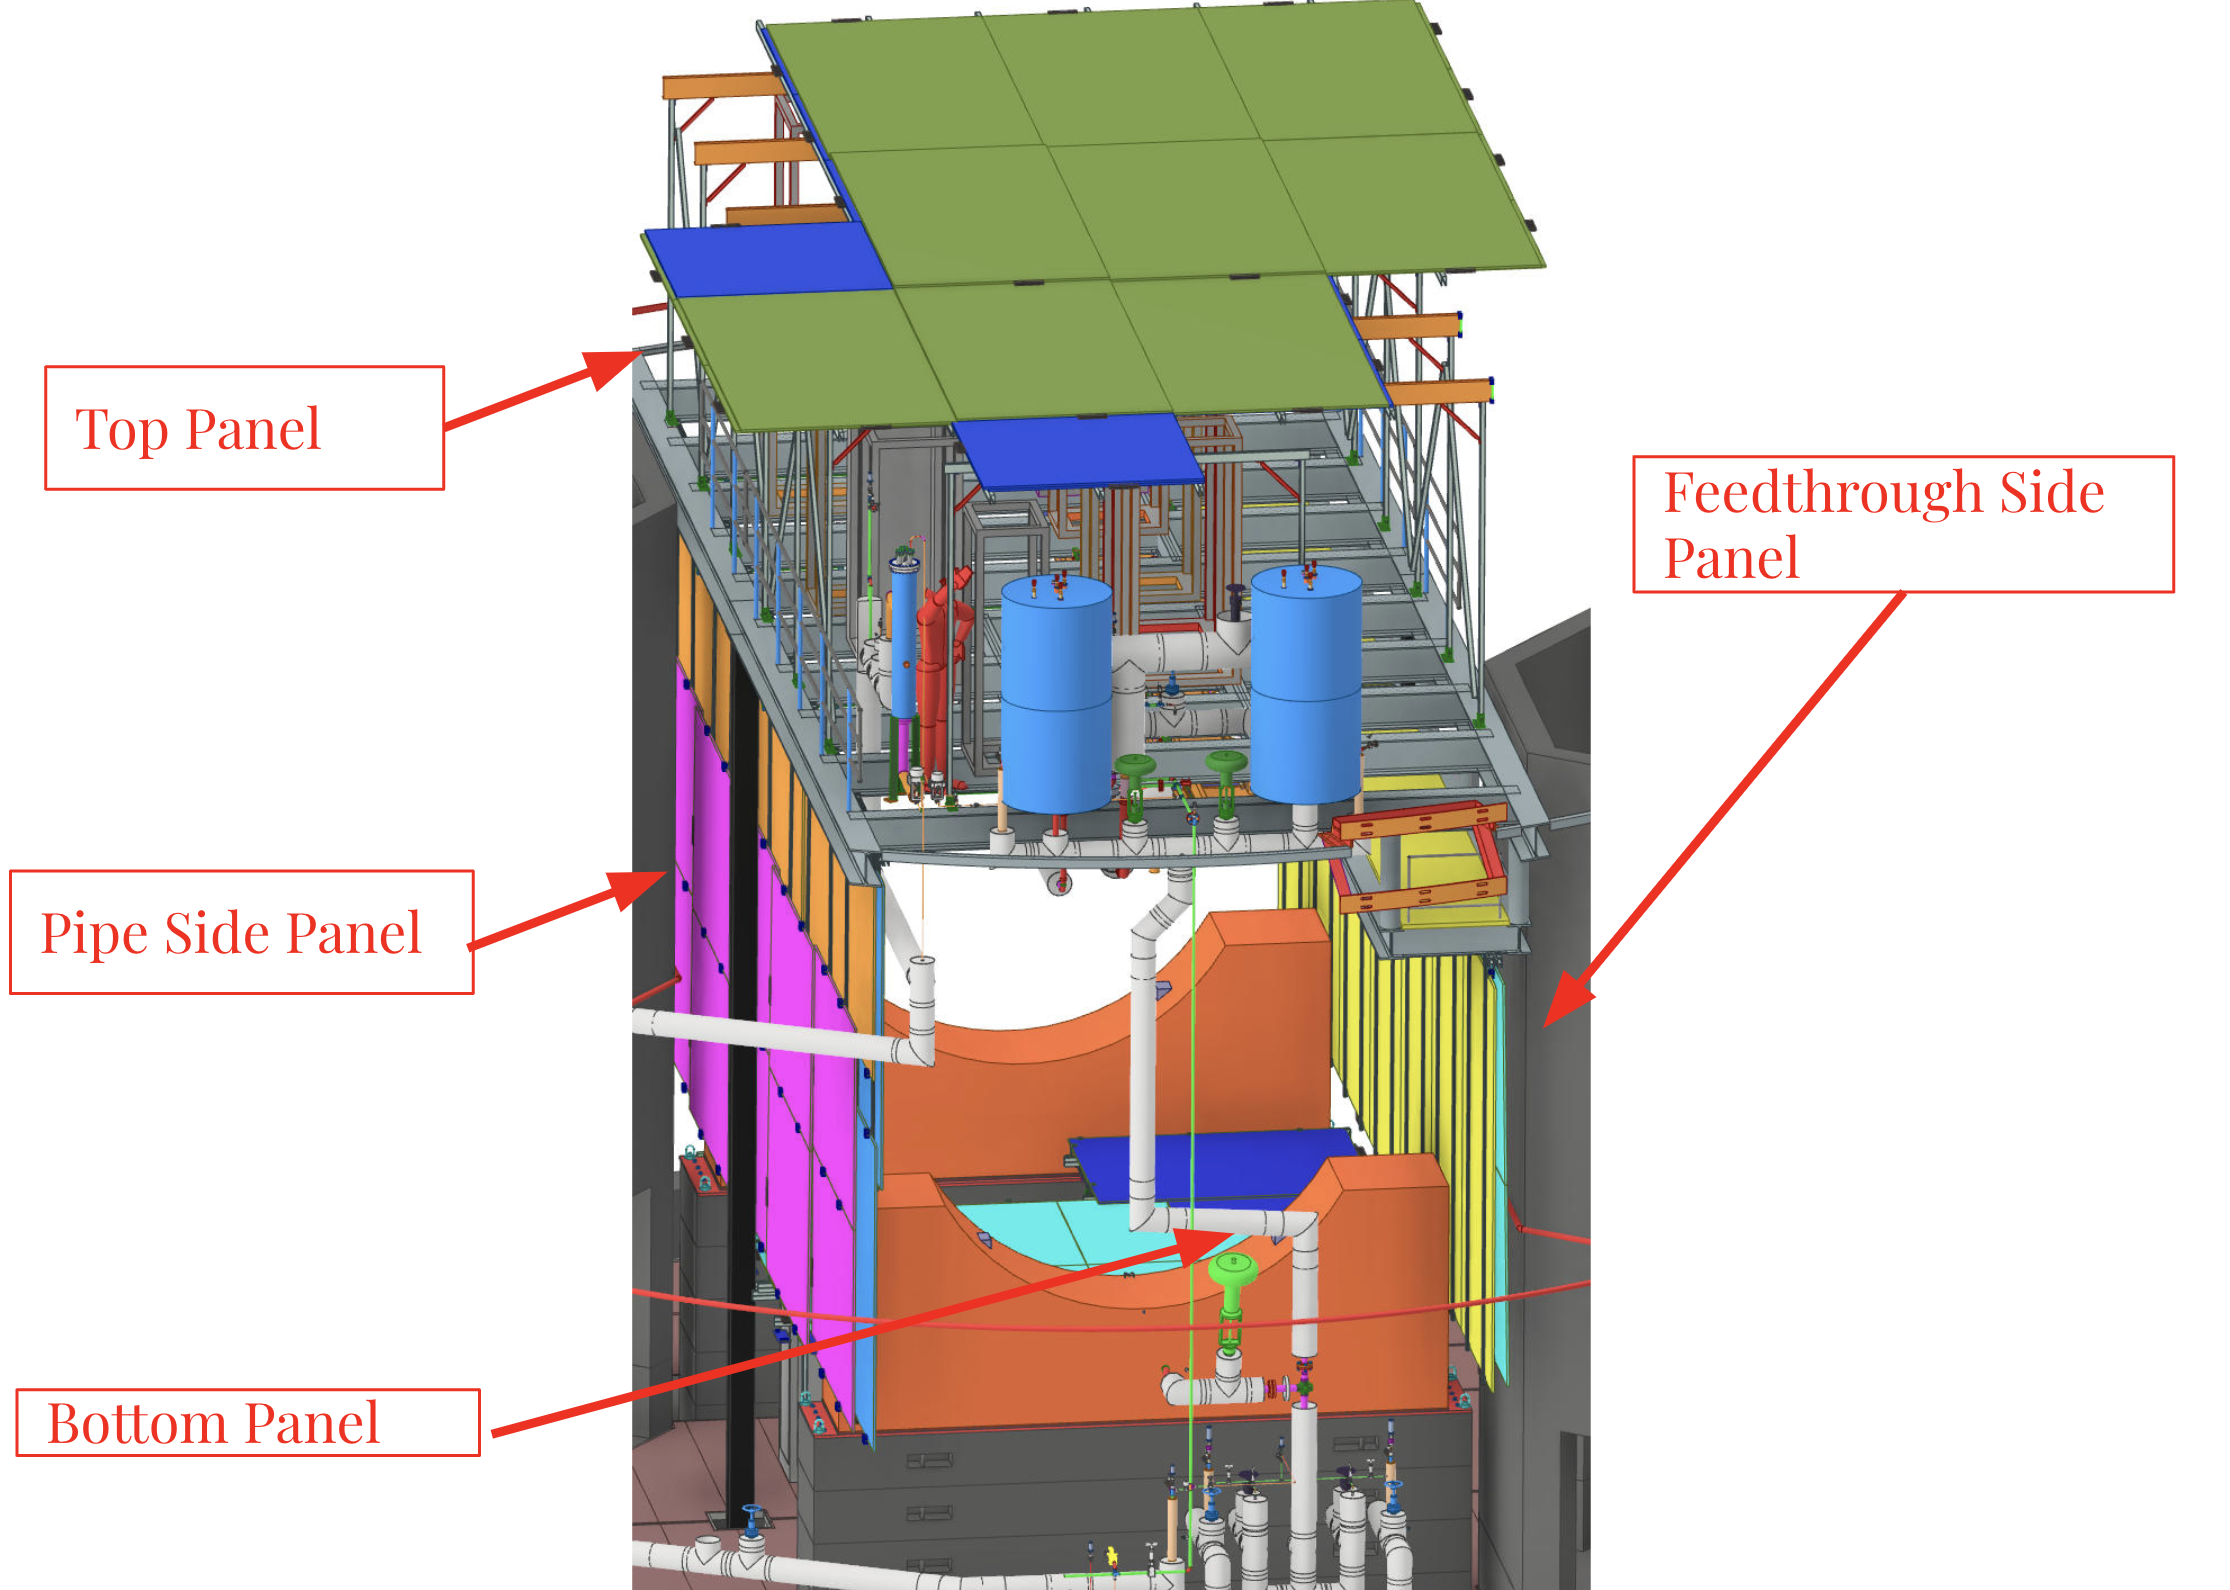
\includegraphics[scale=0.3]{images/CRTScheme}
\caption{Technical drawing of the CRT modules' position in LArTF.}
\label{fig:CRT}
\end{figure}




\subsection{CRT system stability metric: CRT-flash match}
\subsection{CRT system stability metric: CRT-track match}
\subsection{CRT system stability metric: average PE CRT}
\subsection{CRT system stability metric: uncorrected rate}


\subsubsection{Reduced CRT Window and  Uncorrected Rate Definition}\label{sec:RateDef}
%%%%%%%%%%%%%%%%%%%%%%%%%%%%%%%%%%%%%%%%%%%%%%%%%%%%%%%%%%%%%%%%%%%%%%%%%%%%%%%%%
As discussed above, the CRT and TPC readouts are disjoint: data from the two systems are merged at the swizzling stage.  
The CRT reads out data continuously; at the swizzling stage, chunks of CRT readout are merged to the TPC event using the systems timestamps.
Originally, the merged CRT window for each TPC event spanned from -1.94 ms to 4.06 ms around the TPC trigger time. While analyzing data for this work, we noticed that this range is not sufficient to cover cosmic activity for the entire TPC drift time: for example, a cosmic ray crossing the TPC cathode 2.3 ms before the trigger time would be recorded in the TPC drift window, but would be missed in the CRT original readout window. This discovery led to a change in the CRT window merged with the TPC data: analyzers in MCC9.1 can enjoy a new CRT window that spans from -4.2 ms to 5.0 ms around the trigger time. 

In order to avoid swizzling era confusion and  eventual inefficiencies at the window edges,  we used a CRT reduced window per event in this work, which is a consistent subset of the CRT data independent of the swizzling era. We define the reduced CRT window as the CRT data between -1.5 ms to 3.5 ms, see Figure \ref{fig:ReadOutWindow}. 


\begin{figure}[h!]
\centering
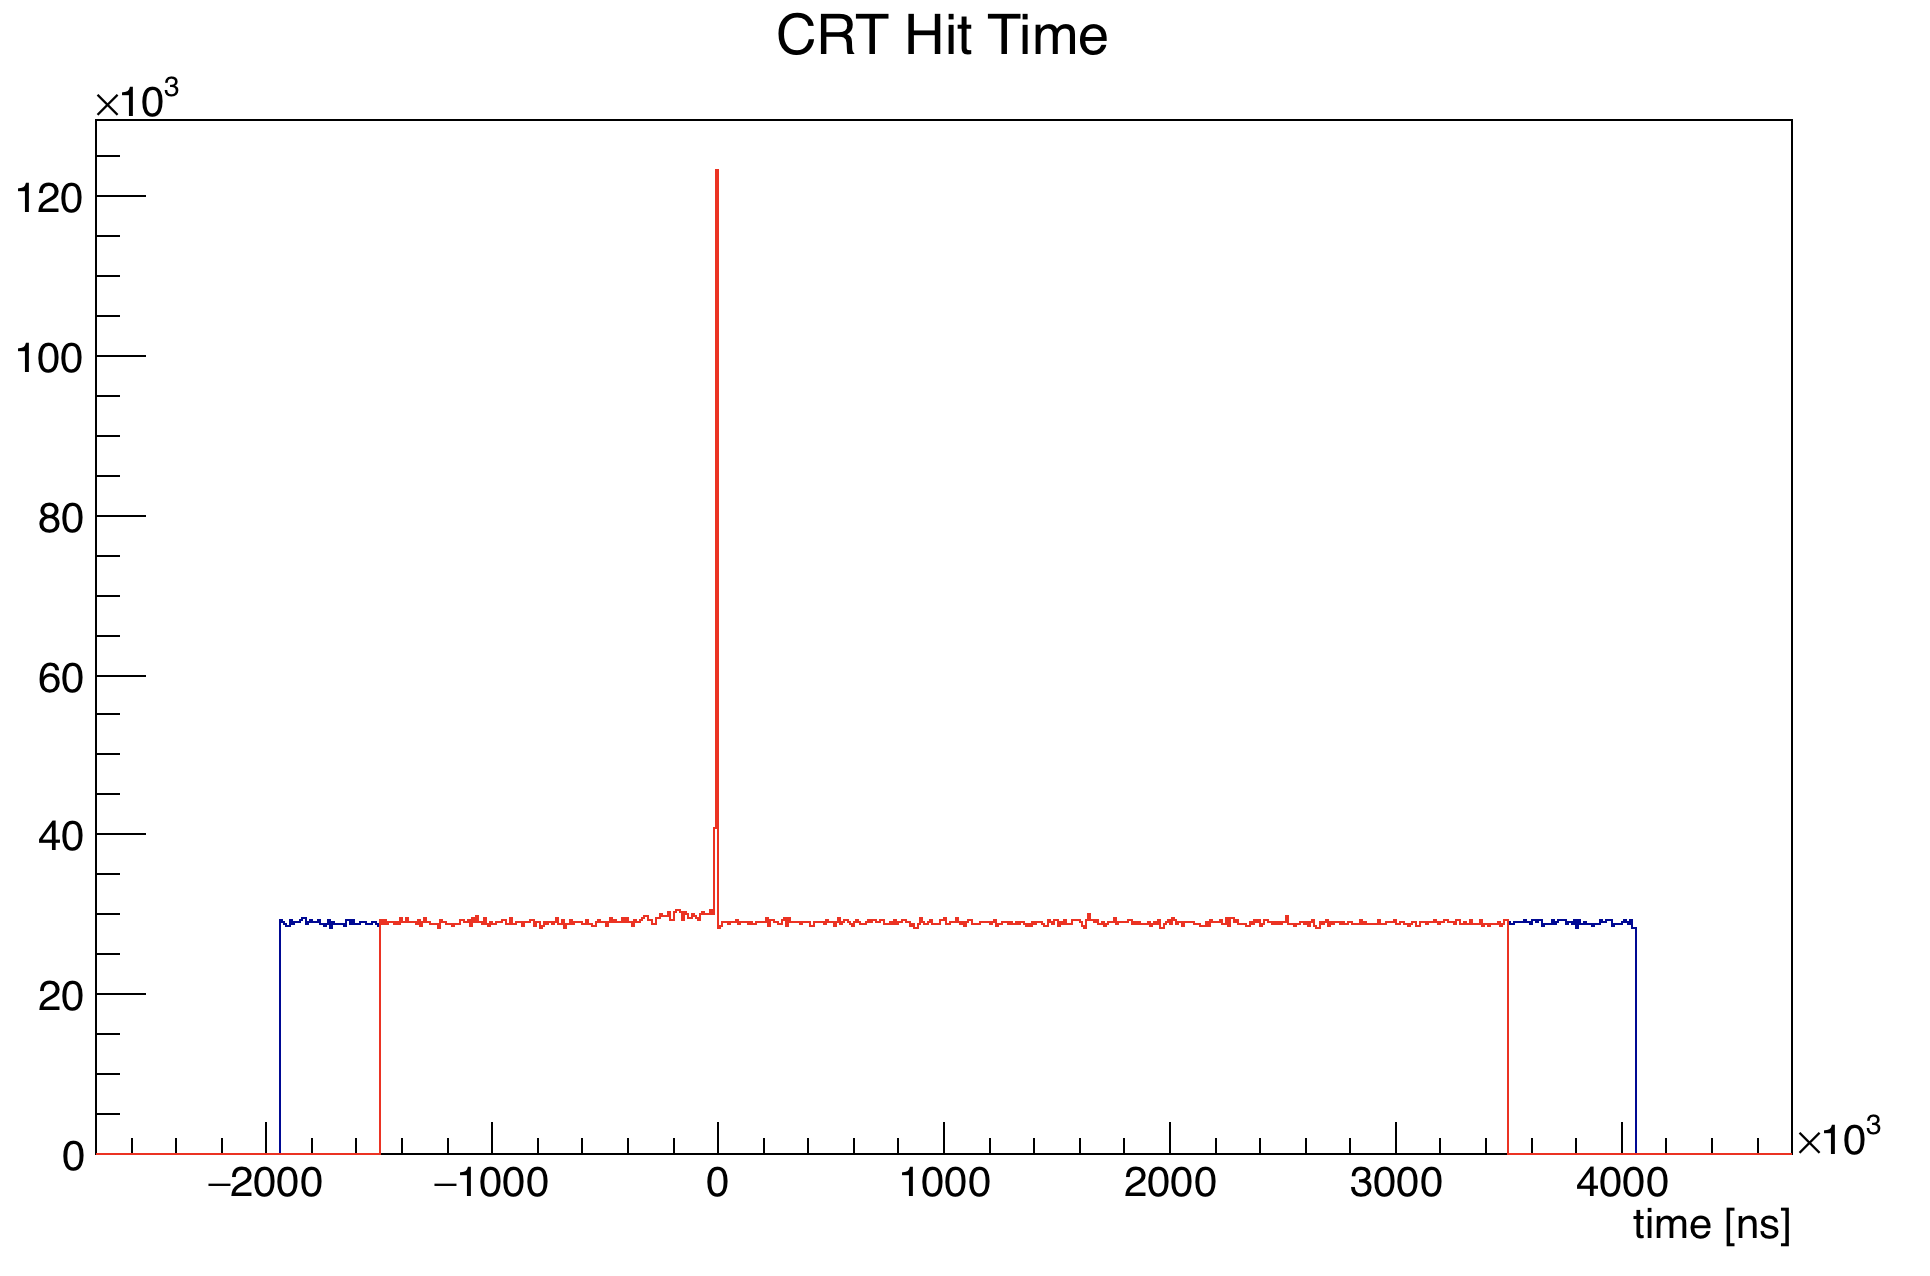
\includegraphics[scale=0.4]{images/window.png}
\caption{CRT readout window in blue, CRT reduced window in red for an arbitrary number of dates in 2018. Data showed here were merged with the original CRT readout window.}
\label{fig:ReadOutWindow}
\end{figure}


We define the uncorrected rate as the ratio between the number of CRT hits in the reduced window and the number of considered events. We calculate the uncorrected rate on each module individually each day. 
Figure \ref{fig:count} shows number of CRT hits in the reduced window for module 11 on 01-01-2018. The integral of this distribution is 19480 hits; since the number of analyzed events that day was 13588, the uncorrected rate is 1.433 $\pm$ 0.016, where the statistical uncertainty is calculated by summing in quadrature the relative poissonian uncertainty on the numerator and denominator.

\begin{figure}[h!]
\centering
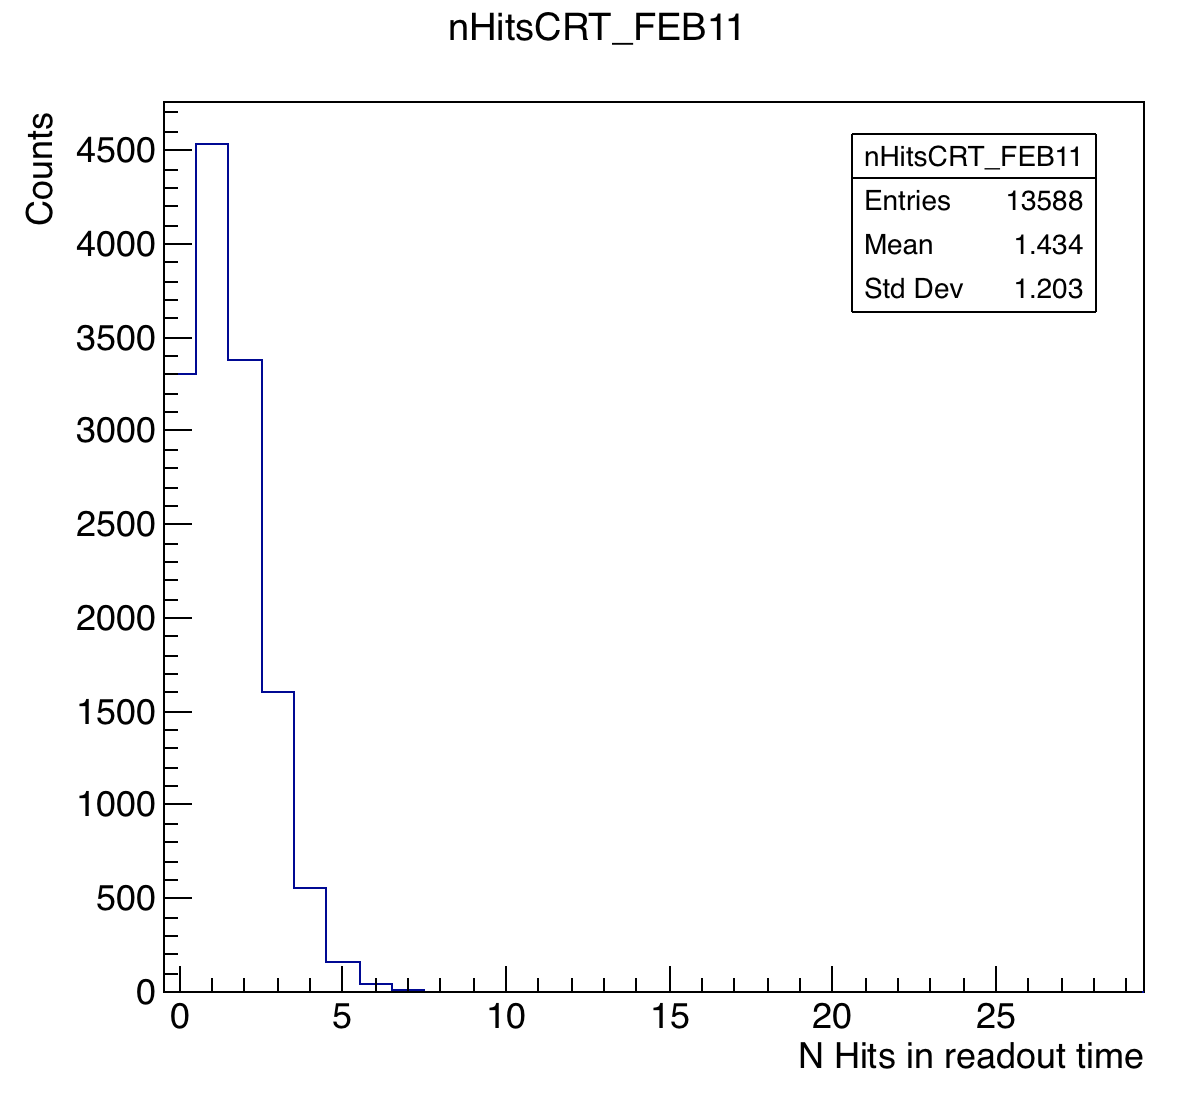
\includegraphics[scale=0.4]{images/count.png}
\caption{CRT hit count on module 11 for 01-01-2018.}
\label{fig:count}
\end{figure}



We analyzed the first two dates of the month for 2018 when BNBExternal data was available. 
As an example, we show the trend for Module 11 in Figure \ref{Annual11_ex}. The blue dotted line represents the average rate for BNBExt; the blue solid lines represents three standard deviations from the mean. All the dates are within three standard deviation from the mean. Analogous plots have been produced for the other 72 modules, leading to the same conclusions regarding the system stability.

\begin{figure}[h!]
\centering
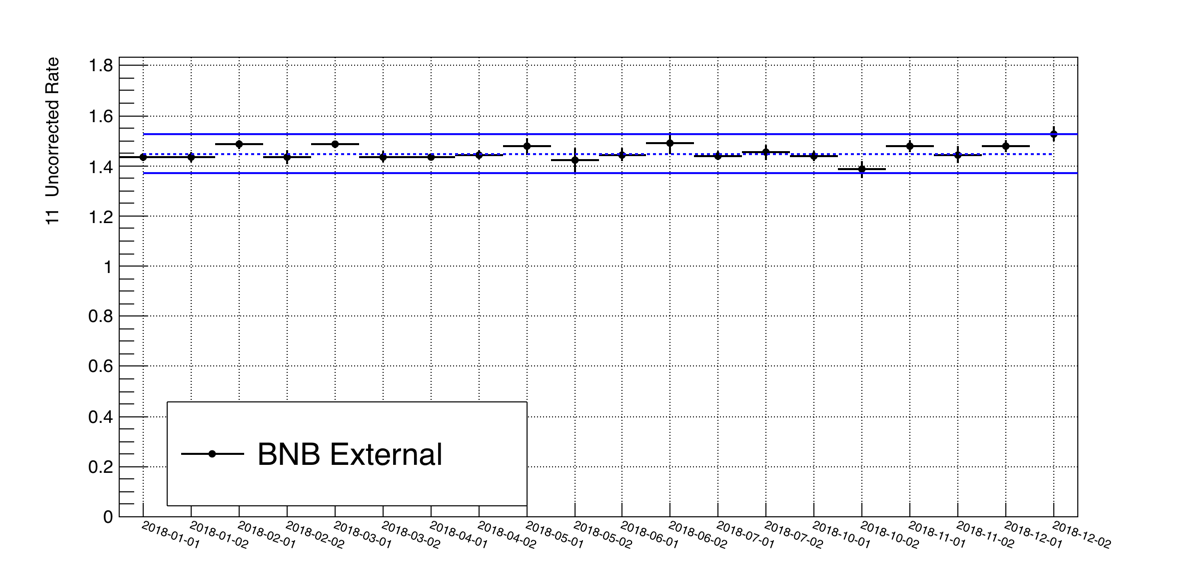
\includegraphics[scale=0.4]{images/hHitsOverEvt_FEB_11.png}
\caption{Uncorrected rate for module 11, 2018 trend: all dates are acceptable.}
\label{Annual11_ex}
\end{figure}


We note here that two hardware changes have happened during the data period deemed usable for physics analysis: a shortening of the CRT run length and the loss of a CRT strip in the top panel. Even if these changes only marginally affect the performances of the CRT, analyzers should be aware of these details when handling CRT data.
%\subsubsection{Shortening of CRT runs}
%\subsubsection{Loss of one top strip}

\clearpage

\appendix
%\input{Appendix}
\newpage
\clearpage


\newpage
%%%%%%%%%%%%%%%%%%%%%%%%%%%%%%%%%
%%  BIBLIOGRAPHY	
%%%%%%%%%%%%%%%%%%%%%%%%%%%%%%%%%
%\bibliographystyle{plain}
%\bibliography{bib}

%\input{reference}


\end{document}